 %%%%%%%%%%%%%%Empieza la presentacion%%%%%%%%%%%%%%%%%%%%%%%%%%%%%%%%%%%%

%\begin{frame}
%\frametitle{Esquema}
 %   \tableofcontents
%\end{frame}



\subsection{Histograma de una imagen digital}

\begin{frame}
\frametitle{Histograma de se\~nales 2D}




\begin{columns}[t]
\begin{column}{5.5cm}

\small
El histograma de una imagen en escala de grises indica el n\'{u}mero de pixels de cada intensidad.

\vspace{0.2cm}

Orden de Matlab (complementa el histograma con una representaci\'{o}n de la escala de grises): \color{red} imhist(im)\color{black}


\lstinputlisting{./Matlab/HistImagen1.m}

\end{column}

\vspace{0.2cm}\begin{column}{2.7cm}

\includegraphics[width=2.2cm,trim={0cm 0cm 0cm 0cm},clip,angle=0]{./Figures/Histograma1_Fig.eps}

\vspace{0.2cm}

\includegraphics[width=2.2cm,trim={0cm 0cm 0cm 0cm},clip,angle=0]{./Figures/Histograma2_Fig.eps}



\end{column}


\hspace{-0.5cm}\begin{column}{3.3cm}

\includegraphics[width=3.3cm,trim={0cm 0cm 0cm 0cm},clip,angle=0]{./Figures/Histograma1_Hist.eps}

\vspace{0.3cm}

\includegraphics[width=3.3cm,trim={0cm 0cm 0cm 0cm},clip,angle=0]{./Figures/Histograma2_Hist.eps}

\end{column}

\end{columns}

\small


\begin{columns}[t]
\begin{column}{12.2cm}
Las im\'{a}genes pueden ser claras u oscuras por si mismas o porque no han sido tomadas con el m\'{e}todo adecuado.

\vspace{0.2cm}

Modificando su histograma, con métodos computacionalmente sencillos, se puede realzar la imagen, aclarar/oscurecer la imagen compensar el brillo.



\end{column}

\end{columns}
\end{frame}


\begin{frame}
\frametitle{Ajuste del histograma}

\small
Lo m\'{a}s sencillo es modificarlo indicando los valores m\'{a}ximos y m\'{i}nimos del histograma de la imagen original y final, y el par\'{a}metro  de la curva que realiza la conversi\'{o}n.

\vspace{0.2cm}

Orden de Matlab: \color{red} imadjust(im,[min$_{orig}$,max$_{orig}$],[min$_{final}$,max$_{final}$],$\alpha$)\color{black}

\begin{columns}[t]
\begin{column}{4.7cm}


\lstinputlisting{./Matlab/HistImagen2.m}

\end{column}

\hspace{-0.1cm}\begin{column}{1.6cm}

\includegraphics[width=1.6cm,trim={0cm 0cm 0cm 0cm},clip,angle=0]{./Figures/Histograma1_Fig.eps}

\vspace{0.2cm}

\includegraphics[width=1.6cm,trim={0cm 0cm 0cm 0cm},clip,angle=0]{./Figures/Histograma1_Hist.eps}

\color{gray}\scriptsize{im1}

\end{column}

\hspace{-0.1cm}\begin{column}{1.6cm}

\includegraphics[width=1.6cm,trim={0cm 0cm 0cm 0cm},clip,angle=0]{./Figures/Histograma2B_Fig.eps}

\vspace{0.2cm}

\includegraphics[width=1.6cm,trim={0cm 0cm 0cm 0cm},clip,angle=0]{./Figures/Histograma2B_Hist.eps}


\color{gray}\scriptsize{im2 ($\alpha=1$, neutro)}

\end{column}

\hspace{-0.1cm}\begin{column}{1.6cm}

\includegraphics[width=1.6cm,trim={0cm 0cm 0cm 0cm},clip,angle=0]{./Figures/Histograma3_Fig.eps}

\vspace{0.2cm}

\includegraphics[width=1.6cm,trim={0cm 0cm 0cm 0cm},clip,angle=0]{./Figures/Histograma3_Hist.eps}


\color{gray}\scriptsize{im3 ($\alpha>1$, oscurece)}
\end{column}


\hspace{-0.1cm}\begin{column}{1.6cm}

\includegraphics[width=1.6cm,trim={0cm 0cm 0cm 0cm},clip,angle=0]{./Figures/Histograma4_Fig.eps}

\vspace{0.2cm}

\includegraphics[width=1.6cm,trim={0cm 0cm 0cm 0cm},clip,angle=0]{./Figures/Histograma4_Hist.eps}


\color{gray}\scriptsize{im4($\alpha<1$, aclara)}
\end{column}

\end{columns}

\end{frame}


\begin{frame}
\frametitle{Ecualizaci\'{o}n del histograma}

Alternativamente, se puede definir el histograma definido en la imagen destino, de forma que se aplique un m\'{e}todo que intente obtenerlo.

\vspace{0.2cm}

Orden de Matlab: \color{red} histeq(im,hist$_{final}$)\color{black}

\begin{columns}[t]
\begin{column}{4.7cm}


\lstinputlisting{./Matlab/HistImagen3.m}

\end{column}

\hspace{-0.1cm}\begin{column}{1.6cm}

\includegraphics[width=1.6cm,trim={0cm 0cm 0cm 0cm},clip,angle=0]{./Figures/Histograma1_Fig.eps}

\vspace{0.2cm}

\includegraphics[width=1.6cm,trim={0cm 0cm 0cm 0cm},clip,angle=0]{./Figures/Histograma1_Hist.eps}

\color{gray}\scriptsize{im1}

\end{column}

\hspace{-0.1cm}\begin{column}{1.6cm}

\includegraphics[width=1.6cm,trim={0cm 0cm 0cm 0cm},clip,angle=0]{./Figures/Histograma5_Fig.eps}

\vspace{0.2cm}

\includegraphics[width=1.6cm,trim={0cm 0cm 0cm 0cm},clip,angle=0]{./Figures/Histograma5_Hist.eps}


\color{gray}\scriptsize{im2 (distribuci\'{o}n uniforme)}

\end{column}

\hspace{-0.1cm}\begin{column}{1.6cm}

\includegraphics[width=1.6cm,trim={0cm 0cm 0cm 0cm},clip,angle=0]{./Figures/Histograma6_Fig.eps}

\vspace{0.2cm}

\includegraphics[width=1.6cm,trim={0cm 0cm 0cm 0cm},clip,angle=0]{./Figures/Histograma6_Hist.eps}


\color{gray}\scriptsize{im3 (histograma prefijado)}
\end{column}



\end{columns}

\end{frame}


\begin{frame}
\frametitle{Binarizaci\'{o}n  del histograma}

\small

Finalmente, el histograma puede ser utilizado para determinar el valor adecuando para binarizar la imagen.

\begin{columns}[t]
\begin{column}{4.7cm}


\lstinputlisting{./Matlab/HistImagen4.m}

\end{column}

\hspace{-0.1cm}\begin{column}{2cm}

\includegraphics[width=2cm,trim={0cm 0cm 0cm 0cm},clip,angle=0]{./Figures/Histograma1_Fig.eps}

\vspace{0.2cm}

\includegraphics[width=2cm,trim={0cm 0cm 0cm 0cm},clip,angle=0]{./Figures/Histograma1_Hist.eps}

\color{gray}\scriptsize{im1}

\end{column}

\hspace{-0.1cm}\begin{column}{2cm}



\includegraphics[width=2cm,trim={0cm 0cm 0cm 0cm},clip,angle=0]{./Figures/HistogramaLast.eps}


\color{gray}\scriptsize{im2 (binarizaci\'{o}n)}

\end{column}

\end{columns}


\end{frame}


\begin{frame}
\frametitle{Visi\'{o}n por computador}


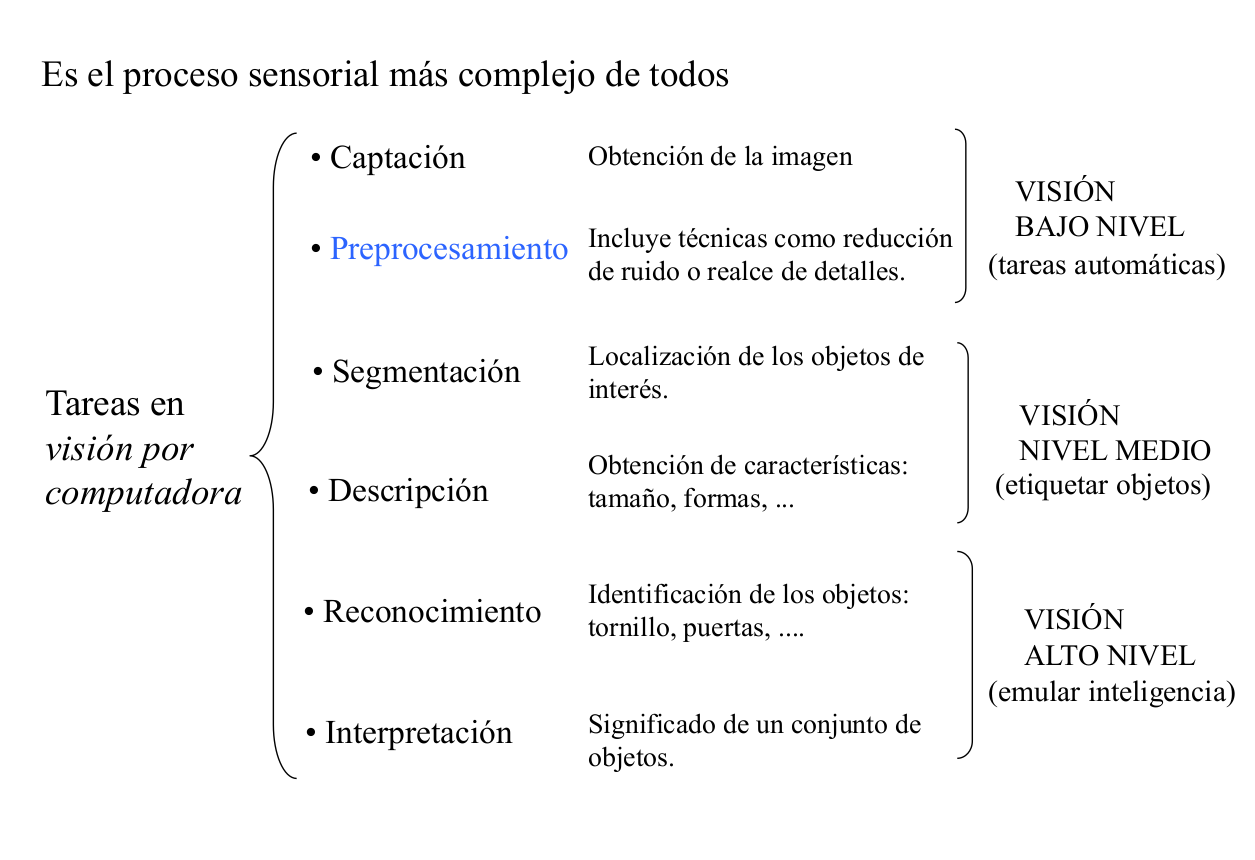
\includegraphics[width=7cm,trim={2cm 2cm 4cm 2cm},clip,angle=90]{./Figures/Clasificacion}


\end{frame}
